% Generated 2020-10-22 16:25:25 +0530
\subsection{CoordinateSystems} \label{sec:CoordinateSystems}


\begin{figure}[ht]
  \centering
    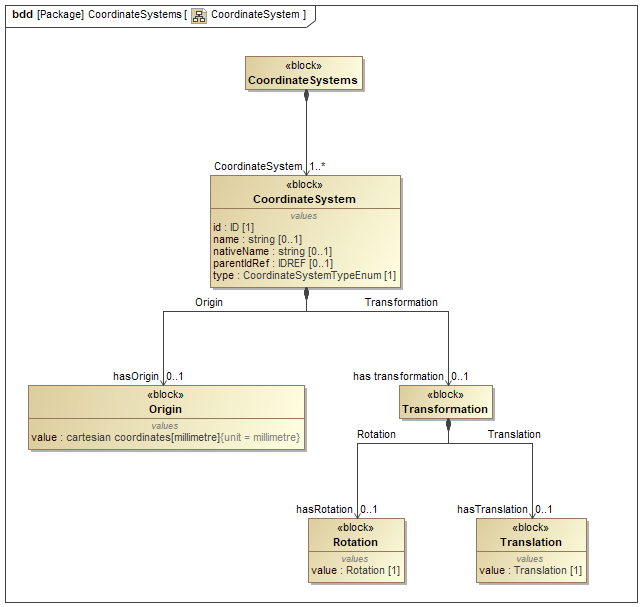
\includegraphics[width=1.0\textwidth]{figures/CoordinateSystem.png}
  \caption{CoordinateSystem Diagram}
  \label{fig:CoordinateSystem}
\end{figure}

\FloatBarrier



\subsubsection{CoordinateSystem}
\label{sec:CoordinateSystem}



A \block{CoordinateSystem} is a reference system that associates a unique set of n parameters with each point in an n-dimensional space. \textit{Ref: ISO 10303-218:2004}


\paragraph{Attributes of CoordinateSystem}\mbox{}
\label{sec:Attributes of CoordinateSystem}

\tbl{Attributes of CoordinateSystem} lists the attributes of \texttt{CoordinateSystem}.

\begin{table}[ht]
\centering 
  \caption{Attributes of CoordinateSystem}
  \label{table:Attributes of CoordinateSystem}
\tabulinesep=3pt
\begin{tabu} to 6in {|l|l|l|} \everyrow{\hline}
\hline
\rowfont\bfseries {Attribute} & {Type} & {Multiplicity} \\
\tabucline[1.5pt]{}
\property{id}[CoordinateSystem] & \texttt{ID} & 1 \\
\property{name}[CoordinateSystem] & \texttt{string} & 0..1 \\
\property{nativeName}[CoordinateSystem] & \texttt{string} & 0..1 \\
\property{parentIdRef}[CoordinateSystem] & \texttt{IDREF} & 0..1 \\
\property{type}[CoordinateSystem] & \texttt{CoordinateSystemTypeEnum} & 1 \\
\end{tabu}
\end{table}
\FloatBarrier


Descriptions for attributes of \block{CoordinateSystem}:

\begin{itemize}

\item \property{id}[CoordinateSystem] : The unique identifier for this element.

\item \property{name}[CoordinateSystem] : The name of the coordinate system.

\item \property{nativeName}[CoordinateSystem] : The manufacturer's name or users name for the coordinate system.

\item \property{parentIdRef}[CoordinateSystem] : A pointer to the \property{id} attribute of the parent \block{CoordinateSystem}.

\item \property{type}[CoordinateSystem] : The type of coordinate system.

\tabulinesep = 5pt
\begin{longtabu} to \textwidth {
    |l|X|}
\caption{CoordinateSystemTypeEnum Enumeration}
\label{enum:CoordinateSystemTypeEnum} \\

\hline
Name & Description \\
\hline
\endfirsthead
\hline
\multicolumn{2}{|c|}{Continuation of Table \texttt{CoordinateSystemTypeEnum} Enumeration} \\
\hline
Name & Description \\
\hline
\endhead
\texttt{WORLD} & stationary coordinate system referenced to earth, which is independent of the robot motion. \textit{ISO 9787:2013}

For non-robotic devices, stationary coordinate system referenced to earth, which is independent of the motion of a piece of equipment. \\ \hline
\texttt{BASE} & coordinate system referenced to the base mounting surface. \textit{ISO 9787:2013}

A base mounting surface is a connection surface between the arm and its supporting structure.\textit{Ref:ISO 9787:2013}

For non-robotic devices, it is the connection surface between the device and its supporting structure. \\ \hline
\texttt{OBJECT} & coordinate system referenced to the object. \textit{ISO 9787:2013} \\ \hline
\texttt{TASK} & coordinate system referenced to the site of the task. \textit{ISO 9787:2013} \\ \hline
\texttt{MECHANICAL\textunderscore INTERFACE} & coordinate system referenced to the mechanical interface. \textit{ISO 9787:2013} \\ \hline
\texttt{TOOL} & coordinate system referenced to the tool or to the end effector attached to the mechanical interface. \textit{ISO 9787:2013} \\ \hline
\texttt{MOBILE\textunderscore PLATFORM} & coordinate system referenced to one of the components of a mobile platform. \textit{ISO 8373:2012} \\ \hline
\texttt{MACHINE} & coordinate system referenced to the home position and orientation of the primary axes of a piece of equipment. \\ \hline
\texttt{CAMERA} & coordinate system referenced to the sensor which monitors the site of the task. \textit{ISO 9787:2013} \\ \hline
\end{longtabu}

\end{itemize}

\paragraph{Elements of CoordinateSystem}\mbox{}
\label{sec:Elements of CoordinateSystem}

\tbl{Elements of CoordinateSystem} lists the elements of \texttt{CoordinateSystem}.

\begin{table}[ht]
\centering 
  \caption{Elements of CoordinateSystem}
  \label{table:Elements of CoordinateSystem}
\tabulinesep=3pt
\begin{tabu} to 6in {|l|l|l|} \everyrow{\hline}
\hline
\rowfont\bfseries {Element Name} & {Type} & {Multiplicity} \\
\tabucline[1.5pt]{}
\block{Origin} & \texttt{Origin} & 0..1 \\
\block{Transformation} & \texttt{Transformation} & 0..1 \\
\end{tabu}
\end{table}
\FloatBarrier


Descriptions for elements of \block{CoordinateSystem}:

\begin{itemize}
\item \block{Origin} : The coordinates of the origin position of a coordinate system.
\item \block{Transformation} :  The process of transforming to the origin position of the coordinate system from a parent coordinate system using \block{Translation} and \block{Rotation}.
\end{itemize}

\subsubsection{CoordinateSystems}
\label{sec:CoordinateSystems}



\block{CoordinateSystems} \glspl{organize} \block{CoordinateSystem} elements for a \block{Component} and its children.


\paragraph{Elements of CoordinateSystems}\mbox{}
\label{sec:Elements of CoordinateSystems}

\tbl{Elements of CoordinateSystems} lists the elements of \texttt{CoordinateSystems}.

\begin{table}[ht]
\centering 
  \caption{Elements of CoordinateSystems}
  \label{table:Elements of CoordinateSystems}
\tabulinesep=3pt
\begin{tabu} to 6in {|l|l|l|} \everyrow{\hline}
\hline
\rowfont\bfseries {Element Name} & {Type} & {Multiplicity} \\
\tabucline[1.5pt]{}
\block{CoordinateSystem} & \texttt{CoordinateSystem} & 1..* \\
\end{tabu}
\end{table}
\FloatBarrier


Descriptions for elements of \block{CoordinateSystems}:

\begin{itemize}
\item \block{CoordinateSystem} : A \block{CoordinateSystem} is a reference system that associates a unique set of n parameters with each point in an n-dimensional space. \textit{Ref: ISO 10303-218:2004}
\end{itemize}

\subsubsection{Origin}
\label{sec:Origin}



The coordinates of the origin position of a coordinate system.


\subsubsection{Rotation}
\label{sec:Rotation}



Rotations about X, Y, and Z axes are expressed in A, B, and C respectively within a 3-dimensional vector. 



\paragraph{Attributes of Rotation}\mbox{}
\label{sec:Attributes of Rotation}

\tbl{Attributes of Rotation} lists the attributes of \texttt{Rotation}.

\begin{table}[ht]
\centering 
  \caption{Attributes of Rotation}
  \label{table:Attributes of Rotation}
\tabulinesep=3pt
\begin{tabu} to 6in {|l|l|l|} \everyrow{\hline}
\hline
\rowfont\bfseries {Attribute} & {Type} & {Multiplicity} \\
\tabucline[1.5pt]{}
\property{value}[Rotation] & \texttt{Rotation} & 1 \\
\end{tabu}
\end{table}
\FloatBarrier


Descriptions for attributes of \block{Rotation}:

\begin{itemize}

\item \property{value}[Rotation] : The value of \block{Rotation} in \texttt{DEGREE\textunderscore 3D}.
\end{itemize}

\subsubsection{Transformation}
\label{sec:Transformation}



 The process of transforming to the origin position of the coordinate system from a parent coordinate system using \block{Translation} and \block{Rotation}.


\paragraph{Elements of Transformation}\mbox{}
\label{sec:Elements of Transformation}

\tbl{Elements of Transformation} lists the elements of \texttt{Transformation}.

\begin{table}[ht]
\centering 
  \caption{Elements of Transformation}
  \label{table:Elements of Transformation}
\tabulinesep=3pt
\begin{tabu} to 6in {|l|l|l|} \everyrow{\hline}
\hline
\rowfont\bfseries {Element Name} & {Type} & {Multiplicity} \\
\tabucline[1.5pt]{}
\block{Translation} & \texttt{Translation} & 0..1 \\
\block{Rotation} & \texttt{Rotation} & 0..1 \\
\end{tabu}
\end{table}
\FloatBarrier


Descriptions for elements of \block{Transformation}:

\begin{itemize}
\item \block{Translation} : Translations along X, Y, and Z axes are expressed as x,y, and z respectively within a 3-dimensional vector. 
\item \block{Rotation} : Rotations about X, Y, and Z axes are expressed in A, B, and C respectively within a 3-dimensional vector. 

\end{itemize}

\subsubsection{Translation}
\label{sec:Translation}



Translations along X, Y, and Z axes are expressed as x,y, and z respectively within a 3-dimensional vector. 


\paragraph{Attributes of Translation}\mbox{}
\label{sec:Attributes of Translation}

\tbl{Attributes of Translation} lists the attributes of \texttt{Translation}.

\begin{table}[ht]
\centering 
  \caption{Attributes of Translation}
  \label{table:Attributes of Translation}
\tabulinesep=3pt
\begin{tabu} to 6in {|l|l|l|} \everyrow{\hline}
\hline
\rowfont\bfseries {Attribute} & {Type} & {Multiplicity} \\
\tabucline[1.5pt]{}
\property{value}[Translation] & \texttt{Translation} & 1 \\
\end{tabu}
\end{table}
\FloatBarrier


Descriptions for attributes of \block{Translation}:

\begin{itemize}

\item \property{value}[Translation] : The value of \block{Rotation} in \texttt{MILLIMETER\textunderscore 3D}.
\end{itemize}
